\documentclass[conference]{IEEEtran}
\IEEEoverridecommandlockouts
% The preceding line is only needed to identify funding in the first footnote. If that is unneeded, please comment it out.
\usepackage{cite}
\usepackage{amsmath,amssymb,amsfonts}
\usepackage{algorithmic}
\usepackage{graphicx}
\usepackage{float}
\usepackage{textcomp}
\usepackage{xcolor}
\def\BibTeX{{\rm B\kern-.05em{\sc i\kern-.025em b}\kern-.08em
    T\kern-.1667em\lower.7ex\hbox{E}\kern-.125emX}}
\begin{document}

\title{A comparison of sampling methods in MCTS\\}
\author{\IEEEauthorblockN{1\textsuperscript{st} Pranav Gopalkrishna}
\IEEEauthorblockA{\textit{School of Electronic Engineering and Computer Science} \\
\textit{Queen Mary University of London}\\
London, UK}
\and
\IEEEauthorblockN{2\textsuperscript{nd} Malo Hamon}
\IEEEauthorblockA{\textit{School of Electronic Engineering and Computer Science} \\
\textit{Queen Mary University of London}\\
London, UK }
\and
\IEEEauthorblockN{3\textsuperscript{rd} Graham Innocent}
\IEEEauthorblockA{\textit{School of Electronic Engineering and Computer Science} \\
\textit{Queen Mary University of London}\\
London, UK}
}

\maketitle

\begin{abstract}
We improve upon the basic MCTS player provided by the TAG framework by experimenting with alternatives to the UCB1 sampling algorithm, using the framework’s implementation of the game Sushi Go! We present our results from experimental exploration of the parameter space of rollout depth for each of these sampling algorithms. To maximise our effectiveness in an expected tournament of agents we also introduce additional techniques such as the All Moves As First heuristic (AMAF), hard pruning and multiple-root averaging and show their effect. An experiment which did not yield the hoped-for performance improvements, biasing rollout by using opponents other than the Random player, is also described. 
\end{abstract}

\begin{IEEEkeywords}
MCTS, UCB1, Thompson Sampling, Bayes-UCB
\end{IEEEkeywords}

\section{Introduction}
Games with a discrete selection of options, such as chess, can be modelled as a branching tree of options, with certain nodes representing an opponent’s moves. An AI controller can therefore be constructed to find an optimal path through this hypothetical tree to try to select the action at each turn most likely to lead to game victory. 

With some games, such as Tic Tac Toe, the game is simple enough that a complete game can be modelled as a shallow tree with sparse branches. Such a tree can be readily explored in full by brute force at each turn using a breadth-first search. However, other games such as Sushi Go! or Chess have a much higher branching factor and more depth to the tree representing a complete game. Exploring such trees by ‘brute force’ methods each turn is not computationally feasible \cite{b1}, so moves are chosen either by heuristics based on domain knowledge of the game, or stochastic methods. In this study, we have focussed on one such method, Monte Carlo Tree Search, and sought to improve upon the performance of the basic implementation provided.

In this study, we implemented new players which used alternative sampling algorithms; Bayes-UCB and Thompson sampling, and the implementation detail of these approaches is explained below. We then describe the experiments we ran to compare their performance with UCB1 to select a final algorithm for tournament submission and choose optimal parameters. This report goes on to detail additional improvements implemented and tested in the construction of our submitted AI player, some with success (AMAF, multiple root averaging and hard pruning). 


\section{TAG}

The experiments described in this report were all implemented using the Tabletop Games Framework \cite{b2}, a set of components implemented in Java which allow researchers to define and run simulated board and card games. Human players or software-defined agents can play the games. The framework allows tournaments of large numbers of matches to be run, thus allowing the study of the properties of new algorithmic game-playing approaches at scale. 

In addition to allowing human players, the framework provides several pre-defined algorithmic agents as described below:-

\begin{enumerate}
\item Random - This player chooses moves at random with uniform distribution. 
\item FirstAction -The 0th element in the list of available actions presented by the Forward Model is always chosen. 
\item OSLA - Calculates the reward of every available action followed by random moves for each opponent, then selects the action with the highest reward.
\item RHEA - This agent implements a Rolling Horizon Evolutionary Agent strategy; an evolutionary algorithm where a  population of action sequences are tested and the most successful ‘bred’ to form the next population. 
\item RMHC - A player based on the Random Mutation Hill Climb. An evolutionary algorithm where an individual sequence of actions is ‘mutated’ to form new individuals.
\item BasicMCTS - A rudimentary implementation of Monte Carlo Tree Search - identifying the best action at each step by sampling many random-walk depth-first searches through the action space. Uses the UCB1 algorithm for sampling. 
\item MCTS - A fully developed, highly configurable implementation of MCTS, is excluded from further study in this report.
\end{enumerate}

The framework also includes several pre-made games ready for experimentation, and one of these, Sushi Go!, was used as the environment in this study. Sushi Go! is a card game for two to five players, which is both stochastic, due to cards being dealt from a shuffled deck, and features imperfect information, due to other players’ hands being hidden.

\section{Background}

\subsection{Handling the exploration vs. exploitation dilemma}
Exploitation refers to making the best decision based on current information, whereas exploration means exploring more uncertain (less sampled) options to gather more information about the environment.

To resolve this, we considered methods in the multi-armed bandit problem framework, i.e. methods that aim to achieve the highest cumulative reward in the long run:

\begin{itemize}
\item Upper confidence bound (UCB) (default)
\item Thompson sampling
\item Bayesian UCB
\end{itemize}

\subsection{Introduction to MCTS}
MCTS is a class of game tree search algorithms that make use of simulated games to evaluate nonterminal states. Simulated games select random actions until a terminal state is reached and the reward is averaged over multiple simulations to estimate the strength of each action\cite{b3}

This approach is justified by the law of large numbers, a statistical law stating that the sample mean asymptotically approaches the true mean as the number of samples tends to infinity. 

\subsection{Explaining the MCTS algorithm}

The core MCTS search loop has four key steps: selection, expansion, rollout/simulation and backpropagation. 

\begin{itemize}
\item Selection decides which state to expand, i.e. which node to explore branches for; the more promising nodes (this promise can be evaluated in different ways) are focused on. Expandability is based also on whether the node has been expanded before or not. Selection stops when an unexpanded node is encountered, after which an action is selected at random (at least in basic MCTS) for the expansion step.
\item Expansion generates a child (usually randomly) of the selected node, i.e. branches the selected node out into a child node obtainable by one of the actions possible from the parent node
\item Rollout/simulation generates a random sequence of actions (i.e. state transitions) originating from the child node of the selected node
\item Backpropagation updates the statistics of the above node (i.e. measures based on its state or position relative to other nodes so far visited) as well as its parents (up to the root node). If we reach a terminal node during rollout where the victory condition can be checked, we use that for the reward of the selected node. Otherwise, we use a heuristic to help evaluate the value of the last state of the rollout and use that for the reward of the selected node
\end{itemize}

\section*{Method}
\subsection{All Moves As First Heuristic (AMAF)}
The AMAF Heuristic was first introduced in the game of Go\cite{b4}, it changes the rollout propagation to include all sibling nodes of the selected node if it matches an action visited during the rollout\cite{b5}. The idea behind this is that it assumes certain moves are strictly good or bad for a particular player\cite{b6}, and therefore the nodes representing these actions should be updated regardless of if they were visited in the particular selection process or not.
We implemented the RAVE implementation of AMAF\cite{b5}, where the AMAF backups and normal backups are computed separately, and merge them using a coefficient: 

\begin{equation}
Q_{RAVE}=\alpha Q_{AMAF}(s, a)) + (1 - \alpha) Q(s, a)
\end{equation}

\begin{equation}
\alpha = \max \{0, \frac{V - N(s)}{V}\}
\end{equation}

The main reasoning behind AMAF is that it reduces the need for exploration as many nodes are explored during the random rollouts\cite{b6}. However this requires the action sequences to be permuted and performed in a different order\cite{b4}. In SushiGo, each action represents selecting a card, so there is no strict requirement for actions to be taken in order, which makes us think implementing RAVE will have a strong impact on MCTS.

\subsection{Thompson Sampling}
As an alternative to the UCB1 tree policy to solve the explore exploit dilemma, we implemented a version of Thompson Sampling. We model each tree node’s value as a distribution, which we can sample and update using Bayesian conjugate priors.

Thompson sampling converges to an optimal minimax tree in certain settings\cite{b7}, and is an efficient way to explore due to the randomization of samples\cite{b7}. In nodes with few visits, the variance is large and therefore samples may vary widely, causing this node to be explored. As the node is explored more, the variance will shrink and the sampled values will get closer to the true value of the node. This should provide a better estimation of the node than UCB1.

We are modelling each node as a Normal distribution with unknown mean and variance:

The variance is modelled as a Gamma Distribution:
\begin{equation}
\tau \sim  Gam(\alpha , \beta )
\end{equation}


The value of the node is modelled as a Normal distribution:
\begin{equation}
Q(s, a) \sim Normal(\overline{x}, \sqrt{\frac{1}{\tau }})
\end{equation}

To efficiently sample from the Gamma and Normal distributions, we utilised the inverse transform sampling trick from [8], which allows us to quickly sample from a distribution using the inverse CDF function of the distribution. Our code implementation uses the SSJ package from the University of Montreal [9].

\subsection{UCB Bayes}
Another alternative to UCB1 we implemented was Bayes-UCB. Bayes-UCB applies Bayesian inference principles to calculate upper confidence bounds for each action's value estimate.\cite{b8}

The Bayes-UCB algorithm assumes a prior distribution over the value of each action. As observations are collected, the posterior distribution is updated, evolving our estimates of the action values. 
Conceptually, this is similar to Thompson sampling, but rewards are treated as a binary state; winning the game or not, rather than a continuous score.


In our implementation, we modelled the reward distribution of each node using a Beta distribution.

\begin{equation}
Q(s, a) \sim  Beta(\alpha , \beta)
\end{equation}

Where ${\alpha}$ and ${\beta}$  are initially 1 to give a uniform distribution, then incremented with wins and losses respectively as observations are collected. 

\subsection{Hard Pruning}
One way of improving the performance of a time-limited tree search algorithm is to selectively skip over unpromising branches. We implemented a variant of the hard-pruning approach described by Hsu \& Perez-Liebana, 2020\cite{b9}

\begin{equation}
remainingNodes = max (\alpha log n, T) 
\end{equation}

${\alpha}$ and T control the minimum number of branches to retain. We sort nodes according to a heuristic based on expected reward, check a node has been visited 20 or more times and mark nodes for skipping until we have remainingNodes left. For large enough values of ${\alpha}$ log n or T, no pruning may occur at a particular node. 

\subsection{Handling Partial Observability}
The basic MCTS algorithm assumes perfect information. Under this assumption, it fixes a root state from which the rest of the search tree is generated. However, it is not possible to fix a root state accurately if we have either (1) partial information about the game state or (2) stochasticity in the initialisation or progression of the game state. In such cases, all we can do is initialise its root with a determinisation, i.e. a possible game state compatible with what we know. To correct for this, we have implemented multi-root MCTS

The core steps of the algorithm are as follows: -\\
\\
function play(player, infoset, n):\\
for n iterations do\\
\indent randomly choose a determinisation $d$ from infoset\\
\indent generate the MCTS search tree for $d$\\
\indent save root, actions taken, children and reward statistics\\
get the average rewards for each first-level action\\
return action with highest average reward\\
\\
\\
We do not modify the MCTS search itself, instead averaging over the results of multiple searches.

\section{Experimental Study}
\subsection{AMAF (RAVE)}
We compared the MCTS Search with and without the RAVE heuristic in SushiGo with 500 games and standard parameters of 100ms of time budget, a maximum tree depth of 30 and a rollout length of 20. We ran this experiment with multiple different values of $amafV$, the hyperparameter which controls how much the AMAF values are used.

\begin{table}[H]
\begin{tabular}{|l|l|l|l|l|}
\hline
amafV & Normal Win rate & RAVE Win rate & Normal M.O.   & RAVE M.O      \\ \hline
50    & 0.48 +/- 0.01   & 0.52 +/- 0.01 & 1.51 +/- 0.01 & 1.48 +/- 0.01 \\ \hline
100   & 0.49 +/- 0.01   & 0.51 +/- 0.01 & 0.51 +/- 0.01 & 1.49 +/- 0.01 \\ \hline
200   & 0.45 +/- 0.01   & 0.55 +/- 0.01 & 1.55 +/- 0.01 & 1.45 +/- 0.01 \\ \hline
300   & 0.51 +/- 0.01   & 0.49 +/- 0.01 & 1.48 +/- 0.01 & 1.50 +/- 0.01 \\ \hline
\end{tabular}
\end{table}

\subsection{Thompson Sampling}
We compared UCB1 to Thompson Sampling in SushiGo with 500 games and our standard parameters. The table below shows the win rate and Mean Ordinal from both agents. Figure \ref{fig:distro1} shows a plot of the score obtained by each agent. In figure \ref{fig:distro2} , we can see the distribution of each child action at the root node after 20, 480, 920 and 1380 iterations of MCTS search. This shows how Thompson Sampling works, at first the actions have a high variance (very wide distributions) and as the number of iterations increases, the variance decreases as the value of the action becomes clearer.
\begin{table}[H]
\begin{tabular}{|l|l|l|}
\hline
\multicolumn{1}{|c|}{\textbf{Agent}} & \multicolumn{1}{c|}{\textbf{Win Rate}} & \multicolumn{1}{c|}{\textbf{Mean Ordinal}} \\ \hline
UCB1& 0.19 +/- 0.01 & 1.80 +/- 0.01\\ \hline
Thompson& 0.81 +/- 0.01& 1.19 +/- 0.01\\ \hline
\end{tabular}
\end{table}

\begin{figure}[H]
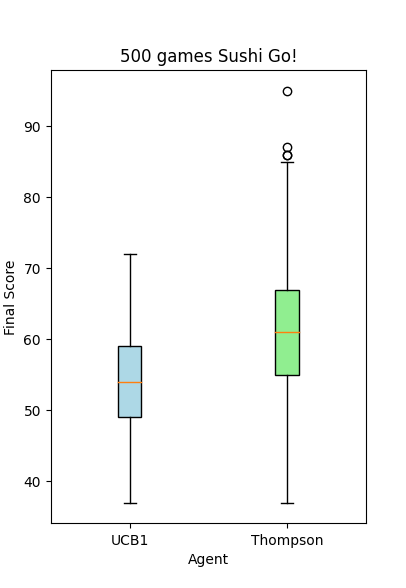
\includegraphics[width=\linewidth]{sushigo-distro.png}
\caption{Score distribution}
\label{fig:distro1}
\end{figure}

\begin{figure}[H]
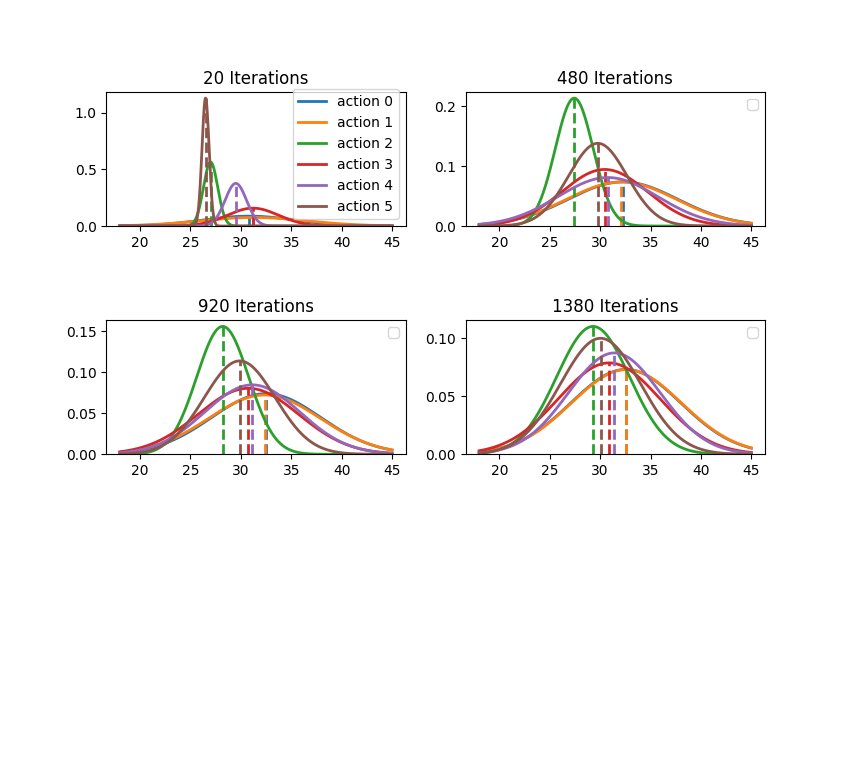
\includegraphics[width=\linewidth]{sushigo-distro2.png}
\caption{Reward distribution}
\label{fig:distro2}
\end{figure}


\subsection{Bayes-UCB}
We compared the Bayes-UCB sampling method to UCB1 in SushiGo with 1000 games, and our standard parameters. The table below shows the win rate and Mean Ordinal from both agents. 

\begin{table}[H]
\begin{tabular}{|l|l|l|}
\hline
\multicolumn{1}{|c|}{\textbf{Agent}} & \multicolumn{1}{c|}{\textbf{Win Rate}} & \multicolumn{1}{c|}{\textbf{Mean Ordinal}} \\ \hline
UCB1                                 & 0.22 +/- 0.01                          & 1.78 +/- 0.01                              \\ \hline
Bayes-UCB                            & 0.78 +/- 0.01                          & 1.22+/- 0.01                               \\ \hline
\end{tabular}
\end{table}

As this result is close to the performance achieved by Thompson sampling above, a further 1000-game trial was run to establish which sampling algorithm would be the best tournament contender for this assignment: -

\begin{table}[]
\begin{tabular}{|l|l|l|}
\hline
\multicolumn{1}{|c|}{\textbf{Agent}} & \multicolumn{1}{c|}{\textbf{Win Rate}} & \multicolumn{1}{c|}{\textbf{Mean Ordinal}} \\ \hline
Bayes-UCB                            & 0.46 +/- 0.01                          & 1.54 +/- 0.01                              \\ \hline
Thompson                             & 0.54 +/- 0.01                          & 1.46+/- 0.01                               \\ \hline
\end{tabular}
\end{table}

\subsection{Hard Pruning}
Early exploration showed that pruning effects were small, so we ran 3000-game tournaments with pruned vs base versions of each algorithm and still saw no statistically significant impact at 95\% confidence.

\subsection{Multi Root}
We ran our multi-root agent against the 1 root version of itself for both the UCB1 and Thompson Sampling tree policy. We ran experiments for 500 games and our standard parameters.

UCB1
\begin{table}[H]
\begin{tabular}{|l|l|l|}
\hline
\textbf{nRoots} & \textbf{Win rate} & \textbf{UCB1 1 root Win Rate} \\ \hline
5               & 66.5\%            & 33.5\%                        \\ \hline
10              & 73.5\%            & 25.5\%                        \\ \hline
\textbf{20}     & \textbf{77.5\%}   & \textbf{22.5\%}               \\ \hline
\end{tabular}
\end{table}

\begin{table}[]
\begin{tabular}{|l|l|l|}
\hline
\textbf{nRoots} & \textbf{Win rate} & \textbf{Thompson 1 root Win Rate} \\ \hline
5               & 43\%              & 58\%                              \\ \hline
10              & 45\%              & 55\%                              \\ \hline
\textbf{20}     & \textbf{51\%}     & \textbf{49\%}                     \\ \hline
\end{tabular}
\end{table}

\section{Discussion}

\subsection{AMAF}
The RAVE heuristic we implemented seemed to have a small effect, having a win rate of 55\% over the normal UCB1 algorithm. This results happens when the amafV value is set to 200, which we deduce is the best value for this configuration. This improvement is likely due to the increased exploration that AMAF offers by updating the value of a node when visited in the rollout.

\subsection{Thompson Sampling}
Our experiments show Thompson Sampling is a clear improvement over UCB1 as a tree policy. It wins over 80\% of the time. The score obtained is significantly higher than UCB1, however interestingly, the variance seems to be similar as we can see from figure[]. Whilst there are more outliers with significantly higher scores, the interquartile range is similar for both UCB1 and Thompson, with Thompson simply scoring higher most of the time. This demonstrates that Thompson Sampling is not only a better Tree Policy for Sushi Go!, but it is also reliable.
We believe this result is due to more efficient exploration of the action space due to the sampling from distributions that Thompson Sampling provides. Thompson Sampling is known to converge faster in cumulative regret than UCB1 [12], which means that it wastes less time visiting bad nodes. In UCB1, exploration is linked to the relative times a node has been visited to its parent, forcing the tree policy to continue visiting nodes with obviously bad values if they have not been visited many times. By contrast, in Thompson Sampling, a node does not have to be visited many times to establish that it does not perform well, whilst still allowing for exploration due to the random sampling.

\subsection{UCB-Bayes}
In the context of Sushi Go!, Bayes-UCB was also a significant improvement upon UCB1 but a 1000-game trial noted above demonstrated that it loses more often than it wins against Thompson sampling playing Sushi Go! under our standard parameters.

We hypothesise that Thompson sampling learns more over time as it is based on a continuous reward (score) rather than the simple binary outcome we used in Bayes-UCB; whether the player wins the game at the end of the rollout or not.

\section{Conclusions and Future Work}
FOR MALO


\begin{thebibliography}{00}
\bibitem{b1} D. Feng, C. Gomes, and B. Selman, "Graph Value Iteration'' https://arxiv.org/pdf/2209.09608.pdf, September 2020.
\bibitem{b2} R.D. Gaina, M. Balla, A Dockhorn, R. Montoliu, D. Perez-Liebana "TAG: A Tabletop Games Framework" http://www.diego-perez.net/papers/TAG\_Tabletop\_Games\_Framework.pdf
\bibitem{b3} Cowling, Powley, and Whitehouse 2012  “Information Set Monte Carlo Tree Search.” IEEE 4, no. ISSN 1943-068X (June). https://eprints.whiterose.ac.uk/75048/1/CowlingPowleyWhitehouse2012.pdf
\bibitem{b4} S. Gelly, D. Silver "Combining online and offline knowledge in UCT" ICML 2007: Proceedings of the 24th international conference on Machine learningJune 2007Pages 273–280https://doi.org/10.1145/1273496.1273531
\bibitem{b5} D. P. Helmbold, A. Parker-Wood "All-Moves-As-First Heuristics in Monte-Carlo Go" https://users.soe.ucsc.edu/~dph/mypubs/AMAFpaperWithRef.pdf
\bibitem{b6} T. Ager "Monte Carlo Tree Search for Go" https://pats.cs.cf.ac.uk/@archive\_file?p=384&n=final&f=1-MCTS\_for\_Go\_Final.pdf\\\&SIG=aaa311815c146f65f167a7318b500dce7143abba70b362835fa0400\\c864e29a7
\bibitem{b7}B. Lindenberg, K Lindahl March 2023 https://arxiv.org/pdf/2303.03348.pdf
\bibitem{b8}E. Kaufmann, O. Cappe and A. Gariver "On Bayesian Upper Confidence Bounds for Bandit Problems" Proceedings of Machine Learning Research http://proceedings.mlr.press/v22/kaufmann12/kaufmann12.pdf
\bibitem{b9}Y. Hsu and D. Perez-Leibana. n.d. “MCTS pruning in Turn-Based Strategy Games.” Queen Mary University of London, London, UK. http://www.diego-perez.net/papers/MCTSPruningTribesAIIDE2020.pdf.
\end{thebibliography}
\vspace{12pt}
\end{document}
